\documentclass[12pt]{article}
\usepackage[top=2.5cm, bottom=2.5cm, left=2.5cm, right=2.5cm]{geometry}
\usepackage[utf8]{inputenc}
\usepackage[icelandic]{babel}
\usepackage[T1]{fontenc}
\usepackage[sc]{mathpazo}
\usepackage[parfill]{parskip}
\usepackage{booktabs}
\usepackage{amsmath}
\usepackage{color}
\usepackage{graphicx}
\usepackage{wrapfig}
\usepackage{subcaption}
\usepackage[pdftex,bookmarks=true,colorlinks=true,linkcolor=blue,urlcolor=blue]{hyperref}

\title{Framleiðsla á humulene í Saccharomyces cerevisiae}
\author{Eiríkur Ernir Þorsteinsson \and Jónas Tryggvi Stefánsson}

\begin{document}

\maketitle

\begin{abstract}
Útdráttur
\end{abstract}

% Myndir verða mikilvægar, fá 2-4
% Byrja á myndunum!
% Hugmynd: Flæðirit yfir virkni reikniritsins

\section{Inngangur}

Þó nokkur fordæmi eru fyrir því að erfðabreyta gersveppum til nota í matvælaiðnaði \cite{dequin2001potential}.

\section{Aðferð}
% Fyrsti textinn sem er skrifaður
% Byrja á undirtitlum
% Mikilvægt að strúktúra málsgreinarnar vel
% Mikilvægt að tengja 
Fyrirsjáanlegar eru tvær aðalleiðir til að hagnýta framleiðslu á humulene í gersvepp.

Fyrri leiðin er að nota erfðabreyttan gersvepp til að gerja bjór í annars hefðbundnu bjórgerðarferli. Sjá \ref{sec:hefdbundid}.

Seinni leiðin er að besta framleiðslu á hreinu humulene, sem síðan væri einangrað. Sjá \ref{sec:optstrain}.

Báðar aðferðir byggjast á greiningu á líkani af gersveppnum.
\subsection{Líkan}
Notast var við Yeast 7 líkanið af gersvepp (\emph{Saccharomyces cerevisiae}), sem sótt var af vefsíðunni \url{http://yeast.sourceforge.net/} og þýtt yfir á Matlab-form sem nýtilegt er með Cobra-pakkanum af Steini Guðmundssyni. Líkanið var valið vegna þess að það er umfangsmikið (m.t.t. fjölda gena og efnahvarfa), með lágt hlutfall blokkaðra efnahvarfa og lágt hlutfall dead-end efna. Önnur líkön gefa betri niðurstöður í sérhæfðum aðstæðum, en þessir eiginleikar Yeast 7 þóttu líklegir til að stuðla að nothæfum niðurstöðum í fyrstu hermunum \cite{heavner2015comparative}.

\subsubsection{Viðbætur á líkani}
Þekkt ensím, (2E,6E)-farnesyl-diphosphate diphosphate-lyase, myndar humulene út frá farnesyl-diphosphate \cite[KEGG: R08373]{Kanehisa01012000}. Farnesyl-diphosphate finnst í terpenoid lífefnasmíðaferlinu \cite[KEGG: rn00900]{Kanehisa01012000}, en bestun á því efnaferli hefur fengið nokkra athygli \cite{BIT:BIT21216,misawa2011pathway,asadollahi2008production}.

Tveimur grundvallar-efnahvörfum var bætt við líkanið til að framleiða humulene úr farnesyl-diphosphate.
Um er að ræða efnahvarf sem framleiðir humulene úr farnesyl-diphosphate annars vegar og exchange-hvarf fyrir humulene-ið hins vegar. Sjá mynd \ref{fig:pathway}

\begin{figure}
\caption[Viðbætur við Yeast 7]{Efnahvörf sem bætt var við Yeast 7 líkanið.}
\label{fig:pathway}
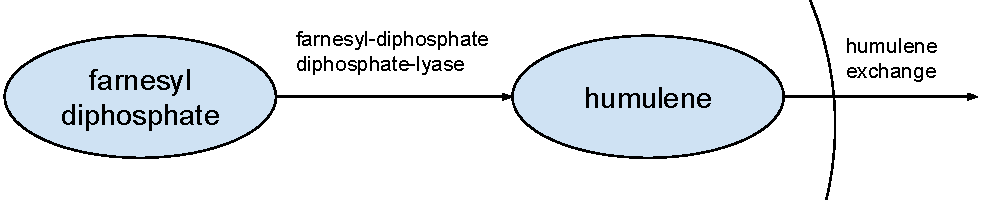
\includegraphics[width=\textwidth]{Pics/HumuleneAddition}
\end{figure}
\subsection{Framleiðsla í hefðbundnu gerjunarferli}
\label{sec:hefdbundid}
\subsubsection{Kolefnisgjafar og gefin skilyrði}
Gerjanlegu sykrurnar í virti eru frúktósi, glúkósi, súkrósi, maltósi og maltótríósi. Þar vega mest hlutverk maltósa, frúktósa og maltótríósa. Maltótríósi er ekki til staðar í Yeast 7 líkaninu og hlutverk annarra kolefnisgjafa er óverulegt, svo til einföldunar voru einungis maltósi og glúkósi tekin til skoðunar. Valin hlutföll eru 1 hlutur glúkósa á móti 2 hlutum maltósa, sem er nálægt meðalhlutföllum þeirra í virti \cite{otter1967determination}. 

Í bjórgerð fer gerjun fram við að mestu leyti loftfirrtar aðstæður. \emph{S. cerevisiae} getur vaxið við slík skilyrði \cite{ishtar2007factors}, en líkanið nær ekki til þeirra.
\subsection{OptStrain}
\label{sec:optstrain}
\begin{figure}
\caption[OptStrain reikniritið]{Skref OptStrain reikniritsins sem lýst er í \ref{sec:optstrain}. Sjá sérstakar viðbætur á mynd \ref{fig:pathway}}
\label{fig:flaedirit}
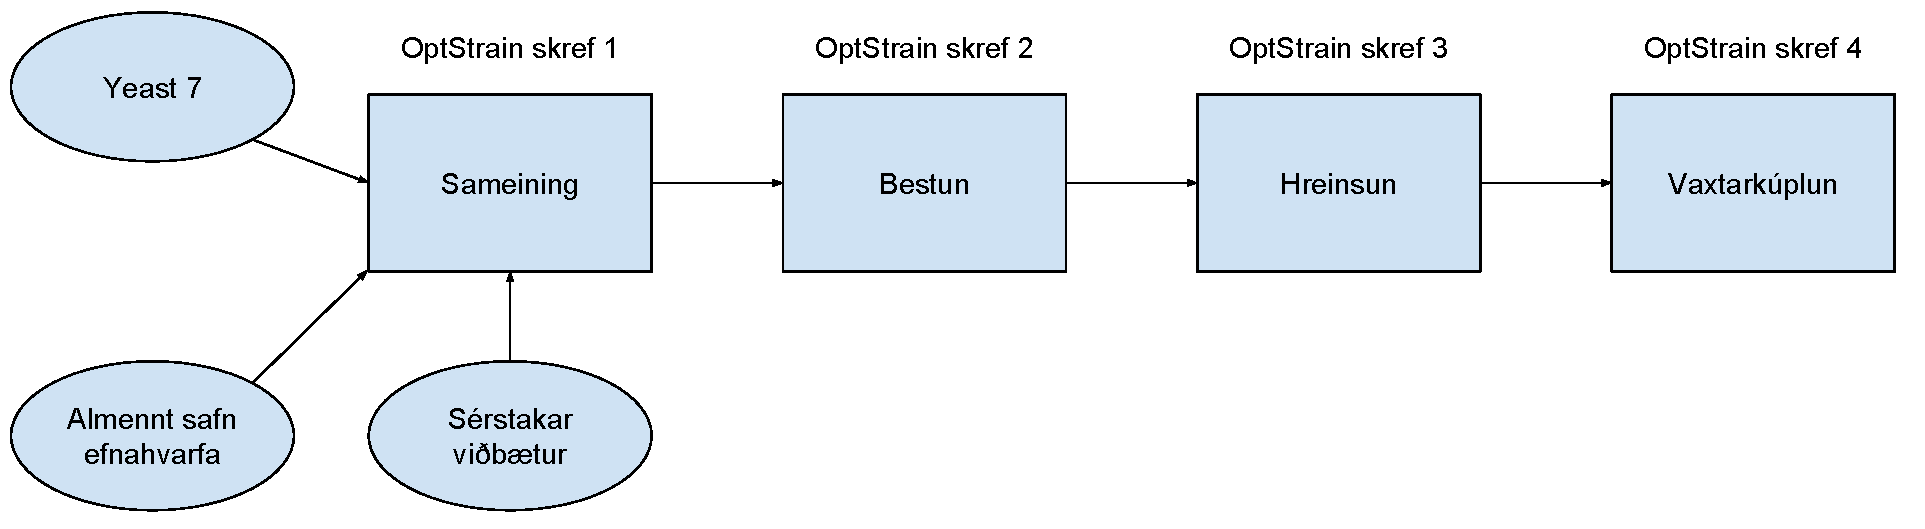
\includegraphics[width=\textwidth]{Pics/OptStrainOverview}
\end{figure}
\subsubsection{Almenn lýsing}
\subsubsection{Útfærsla}

\section{Niðurstöður}

Mikilvæg efni eru: ethanol, isoamyl acetate (bananabragð), glycerol (sæta), urea (óbragð) \cite{dequin2001potential}.

% Undirtitlar hér líka

\begin{figure}
\caption[Áhrif humulene á hefðbundna gerjun]{Yfirlit yfir áhrif humulene-framleiðslu á hefðbundna gerjun}
\centering
\begin{subfigure}[b]{0.45\textwidth}
\caption{Hámarksflæði með og án bestunar á humulene-framleiðslu}
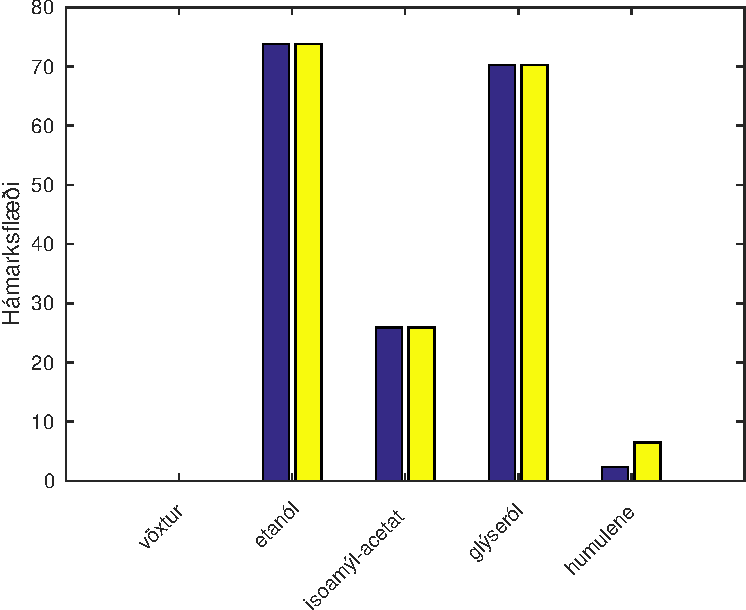
\includegraphics[width=\textwidth]{Pics/BrewingMetMaxFlow}
\end{subfigure}
\hspace{0.5cm}
\begin{subfigure}[b]{0.45\textwidth}
\caption{Áhrif humulene-framleiðslu á markfallsgildi}
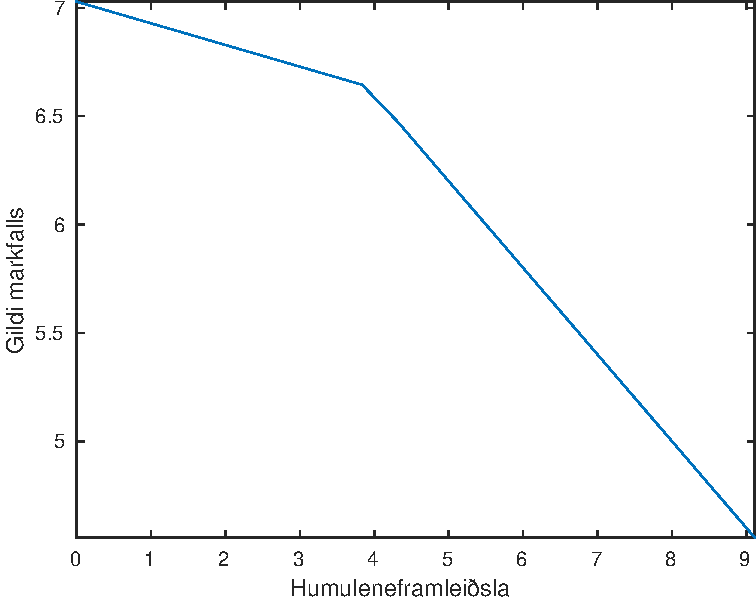
\includegraphics[width=\textwidth]{Pics/BrewingRobustnessAnalysis}
\end{subfigure}
\end{figure}

\section{Samantekt}
% Byrjar oftast eins: Here we set out to...

% \paragraph{Samantekt á niðurstöðum}
% \paragraph{Hvernig falla niðurstöðurnar að öðrum þekktum niðurstöðum}
% Ræða hvern undirtitil í niðurstöðu-hlutanum sérstaklega
% Aftur samantekt á síðustu málsgreinum, summary of impact

\appendix
%%%%%%%%%%%%%%
% HEIMILDASKRÁ
%%%%%%%%%%%%%%
\bibliographystyle{plain}
\bibliography{bioinfo.bib}

\end{document}